\documentclass[a4paper,11pt]{article}
\usepackage[left=2.5cm, right=2.5cm, top=1.5cm, bottom=1.5cm]{geometry}
\usepackage{graphicx}
\usepackage{amssymb}
\usepackage{amsmath}
\usepackage{xcolor}
\usepackage[active,tightpage]{preview}
\usepackage{hyperref}
\usepackage{pythonhighlight}

\hypersetup{ %color attributes of citation, link, etc.
    colorlinks=true,
    linkcolor=blue,
    filecolor=gray,
    urlcolor=blue,
    citecolor=blue,
}

\setlength{\parindent}{0pt}

\renewcommand{\PreviewBorder}{1in}
\newcommand{\Newpage}{\end{preview}\begin{preview}}
\newcommand{\matlab}{\textsc{Matlab}} %very important and totally necessary addition
\newcommand{\parallelsum}{\mathbin{\!/\mkern-5mu/\!}}

\newcommand\Item[1][]{%
  \ifx\relax#1\relax  \item \else \item[#1] \fi
  \abovedisplayskip=0pt\abovedisplayshortskip=0pt~\vspace*{-\baselineskip}}

%'codify' text for snippets
\usepackage{xcolor}
\definecolor{codegray}{gray}{1}
\newcommand{\code}[1]{\colorbox{codegray}{\texttt{#1}}}


\graphicspath{ {./images/} }
           
\begin{document}
\begin{preview}
\title{\LARGE{\textbf{ENGR222 Assignment 2}}}
\author{Niels Clayton : 300437590}
\date{}
\maketitle
\hrule

\begin{enumerate}
\item Multiple Integrals 

\begin{enumerate}
    \item Evaluate the integral of $f (x, y, z) = xyz$ over the region:
    $$ G = \{ (x,y,z):xy \leq z \leq 1, \; 0 \leq x \leq y, \; 0 \leq y \leq 1 \} $$

    \begin{align*}
        \iiint_G f(x,y,z)dV &= \int_{0}^{1} \int_{0}^{y} \int_{xy}^{1} xyz\; dz\,dx\,dy\\
        &= \int_{0}^{1} \int_{0}^{y} xy \Big|\frac{z^2}{2}\Big|_{z=xy}^{z = 1}\;dx\,dy\\
        &= \int_{0}^{1} \int_{0}^{y} xy \left( \frac{1}{2} - \frac{x^2y^2}{2} \right)\;dx\,dy\\
        &= \int_{0}^{1} \int_{0}^{y} \frac{1}{2} (xy - x^3y^3) \;dx\,dy\\
        &= \int_{0}^{1} \frac{1}{2} \Big| \frac{x^2 y}{2} - \frac{x^4y^3}{4} \Big|_{0}^{y} \;dy\\
        &= \frac{1}{8} \Big| \frac{y^4}{2} - \frac{y^8}{8}\Big|_{y = 0}^{y = 1}\\
        &= \frac{1}{8} \left( \frac{1}{2} - \frac{1}{8}\right) = \frac{3}{64} \\
    \end{align*}

    \item Using spherical coordinates, determine the integral of $f (x,y,z)= x$ over the region $G$ described by the inequalities $ x,y,z \geq 0 $ and $ x^2 + y^2 + z^2 \leq 1 $\\
    
    In spherical ordinates we have: \\$ f(r, \theta, \phi) = r\cos(\theta) \sin(\phi) $ for $G = \{ (r, \theta, \phi): 0 \leq r \leq 1, \; 0 \leq \theta \leq \frac{\pi}{2}, \; 0 \leq \phi \leq \frac{\pi}{2} \}$

    \begin{align*}
        \iiint_G f(r, \theta, \phi)dV &= \int_{0}^{1} \int_{0}^{\frac{\pi}{2}} \int_{0}^{\frac{\pi}{2}} r\cos(\theta) \sin(\phi) \; d\phi\,d\theta\,dr\\
        &= \int_{0}^{1} r \; dr \int_{0}^{\frac{\pi}{2}} \cos(\theta) \;d\theta \int_{0}^{\frac{\pi}{2}} \sin(\phi) \; d\phi\\
        &= \frac{r^2}{2}\Big|_{r=0}^{r=1} \times \sin(\theta)\Big|_{\theta = 0}^{\theta = \frac{\pi}{2}} \times -\cos\phi\Big|_{\phi=0}^{\phi=\frac{\pi}{2}}\\
        &= \frac{1}{2} \times 1 \times 1 = \frac{1}{2}
    \end{align*}

    \item Calculate the integral of $f(x,y) = y^{-2}e^{-x}$ over the region
    $$ R = \{ (x,y): x \in [0,\infty], y \in [2,\infty]\} $$

    \begin{align*}
        \iint_R f(x,y) \; dA &= \int_{2}^{\infty} y^{-2} \;dy \int_{0}^{\infty} e^{-x} \;dx\\
        &= -\frac{1}{y}\Big|_{2}^{\infty}  \times -e^{-x}\Big|_{0}^{\infty} \\
        &= \left( 0 + \frac{1}{2} \right) \times \left( 0 + 1 \right)\\
        &= \frac{1}{2}
    \end{align*}

    \item Determine the centroid of the two dimensional object described in polar coordinates by
    $$ R = \{ (r, \theta): 0 \leq r \leq \theta, \theta \in [0, 2\pi] \} $$

    \begin{align*}
        \bar{x} &= \frac{1}{\mathrm{area \; of \; R}} \iint_{R}r^2\cos(\theta) \; dr\; d\theta\\
        \bar{y} &= \frac{1}{\mathrm{area \; of \; R}} \iint_{R}r^2\sin(\theta) \; dr\; d\theta\\\\
        \mathrm{area \; of \; R} &= \int_{\theta_0}^{\theta_1}\frac{1}{2}r^2 \; d \theta\\
        &= \int_{0}^{2\pi}\frac{1}{2} \theta^2 \; d \theta\\
        &= \frac{1}{6} \theta^3 \Big|_{0}^{2\pi}\\
        &= \frac{1}{6} 8\pi^3 = \frac{4\pi^3}{3}\\\\
        \iint_{R}r^2\cos(\theta) \; dr\; d\theta &= \int_{0}^{2\pi}\int_{0}^{\theta} r^2\cos(\theta) \; dr\; d\theta\\
        &= \frac{1}{3} \int_{0}^{2\pi} r^3\cos(\theta)\Big|_{0}^{\theta} \; d\theta \\
        &= \frac{1}{3} \int_{0}^{2\pi} \theta^3\cos(\theta) \; d\theta \\
        &= \frac{1}{3}(12\pi^2) = 4\pi^2\\\\
        \iint_{R}r^2\sin(\theta) \; dr\; d\theta &= \int_{0}^{2\pi}\int_{0}^{\theta} r^2\sin(\theta) \; dr\; d\theta\\
        &= \frac{1}{3} \int_{0}^{2\pi} r^3\sin(\theta)\Big|_{0}^{\theta} \; d\theta \\
        &= \frac{1}{3} \int_{0}^{2\pi} \theta^3\sin(\theta) \; d\theta \\
        &= \frac{1}{3}(12\pi - 8\pi^3)\\\\
        \bar{x} &= \frac{1}{\frac{4\pi^3}{3}}4\pi^2 = \frac{3}{4\pi^3}4\pi^2 \\
        &= \frac{3}{\pi} \approx 0.955\\\\
        \bar{y} &= \frac{1}{\frac{4\pi^3}{3}}\frac{(12\pi - 8\pi^3)}{3} = \frac{3}{4\pi^3}\frac{(12\pi - 8\pi^3)}{3}\\\\
        &= -1.696
    \end{align*}
    The centroid can be found at $(x,y)=(0.955, -1.696)$\\

\end{enumerate}

\item Vector Fields

\begin{enumerate}
    \item Calculate the divergence of the vector field $\textbf{F} = x^2y^3z^4 \textbf{i} - xyz \textbf{j} + (x+y+z) \textbf{k}$
    
    \begin{align*}
        \mathrm{div} \; \textbf{F} &= \frac{\partial f}{\partial x } + \frac{\partial g}{\partial y } + \frac{\partial h}{\partial z }\\
        &= 2xy^3z^4 - xz + 1
    \end{align*}

    \item Calculate the curl of the vector field $\textbf{F} = x^2y^3z^4 \textbf{i} - xyz \textbf{j} + (x+y+z) \textbf{k}$
    
    \begin{align*}
        \mathrm{curl} \; \textbf{F} &= \left( \frac{\partial h}{\partial y} - \frac{\partial g}{\partial z} \right) \textbf{i} - \left( \frac{\partial f}{\partial z} - \frac{\partial h}{\partial x} \right) \textbf{j} + \left( \frac{\partial g}{\partial x} - \frac{\partial f}{\partial y} \right) \textbf{k}\\\\
        &= \left( 1 + xy \right) \textbf{i} - \left( 4x^2y^3z^3 - 1 \right) \textbf{j} - \left( yz + 3x^2y^2x^4 \right) \textbf{k}\\
    \end{align*}

    \item Determine the gradient field of $\phi(x,y,z) = xz^2 + sin(y)e^x$
    
    \begin{align*}
        \nabla \phi &= \frac{\partial \phi}{ \partial x} \textbf{i} + \frac{\partial \phi}{ \partial y} \textbf{j} + \frac{\partial \phi}{ \partial z} \textbf{k}\\\\
        &= \left(z^2 + sin(y)e^x\right) \textbf{i} + \left( \cos(y)e^x \right) \textbf{j} + \left( 2xz \right) \textbf{k}\\
    \end{align*}

    \item Calculate the Laplacian of $\phi(x,y,z) = xz^2 + sin(y)e^x$ 
    
    \begin{align*}
        \nabla \phi ^2 &= \frac{\partial^2 \phi}{ \partial x^2} + \frac{\partial^2 \phi}{ \partial y^2} + \frac{\partial^2 \phi}{ \partial z^2} \\\\
        &= \sin(y)e^x -\sin(y)e^x + 2x\\
        &=2x
    \end{align*}

\end{enumerate}

\item Line integrals

\begin{enumerate}
    \item Calculate the value of the line integral $\int_C f \; ds$ where
    $$ f(x,y,z) = \frac{y}{x}e^z $$
    and $C$ is described by 
    $$(x,y,z) = (2t, \; t^2, \; ln(t)) \;\;\mathrm{for} \;\; t \in [1,4]$$

    \begin{align*}
        \int_C f(x,y,z)ds &= \int_{a}^{b} f(x(t), y(t), z(t)) \;||r'(t)|| \;dt \\\\
        f(2t, t^2, ln(t)) &= \frac{t^2}{2t}e^{ln(t)} \\
        &= \frac{t^2}{2}\\\\
        r'(t) &= \frac{dx}{dt} \textbf{i} + \frac{dy}{dt} \textbf{j} +  \frac{dz}{dt} \textbf{k}\\
        &= 2 \textbf{i} + 2t \textbf{j} + \frac{1}{t} \textbf{k}\\\\
        ||r'(t)|| &= \sqrt{\frac{dx}{dt}^2  + \frac{dy}{dt}^2 +  \frac{dz}{dt}^2}\\
        &= \sqrt{4 + 4t^2 + \frac{1}{t^2}}\\
        &=\sqrt{\frac{4t^4 + 4t^2 + 1}{t^2}}\\
        &=\frac{\sqrt{4t^4 + 4t^2 + 1}}{t}\\
        &= \frac{\sqrt{(2t^2 + 1)^2}}{t}\\
        &= \frac{(2t^2 + 1)}{t}\\\\
        \int_C f(x,y,z)ds &= \int_{1}^{4} \frac{t^2}{2} \frac{(2t^2 + 1)}{t} \; dt\\
        &= \int_{1}^{4} \frac{t(2t^2 + 1)}{2} \; dt\\
        &= \int_{1}^{4} \frac{(2t^3 + t)}{2} \; dt\\\\
        &= \frac{t^4}{4}+\frac{t^2}{4} \Big|_{1}^{4}\\
        &= \frac{4^4}{4} + \frac{4^2}{4}- \frac{1^4}{4} - \frac{1^2}{4}\\
        &= \frac{135}{2} = 67.5\\
    \end{align*}

    \item Calculate the value of the line integral $\int_C \textbf{F} \cdot \; d \textbf{r}$ where
    $$ \textbf{F}(x,y,z) = x \textbf{i} - e^z \textbf{j} + y \textbf{k} $$
    and $C$ is described by
    $$(x,y,z) = (2t, \; t^2, \; ln(t)) \;\;\mathrm{for} \;\; t \in [1,4]$$

    \begin{align*}
        \int_C \textbf{F} \cdot \; d \textbf{r} &= \int_a^b \textbf{F}(\textbf{r}(t)) \cdot \textbf{r}' (t) \; dt\\\\
        \textbf{F}(\textbf{r}(t)) &= 2t \textbf{i} - e^{ln(t)} \textbf{j} + t^2 \textbf{k}\\
        &= 2t \textbf{i} - t \textbf{j} + t^2 \textbf{k}\\\\
        \textbf{r}' (t) &= \frac{dx}{dt} \textbf{i} + \frac{dy}{dt} \textbf{j} +  \frac{dz}{dt} \textbf{k}\\
        &= 2 \textbf{i} + 2t \textbf{j} + \frac{1}{t} \textbf{k}\\\\
        \textbf{F}(\textbf{r}(t)) \cdot \textbf{r}' (t) &= 5t - 2t^2 \\\\
        \int_C \textbf{F} \cdot \; d \textbf{r} &= \int_1^4 5t - 2t^2 \; dt\\
        &= \frac{5}{2}t^2 - \frac{2}{3}t^3 \; \Big|_{1}^{4}\\
        &= \left(\frac{5}{2} \times 16\right) - \left(\frac{2}{3} \times 64 \right) - \left(\frac{5}{2}\right) + \left(\frac{2}{3} \right)\\
        &= -4.5
    \end{align*}

    \item Calculate the value of the line integral $\int_C \textbf{F} \cdot \; d \textbf{r}$ where $F$ is the gradient field of $$ \phi = \cos(x \sin(ye^z) ) $$
    and $C$ is described by the vector-valued function 
    $$ \textbf{r}(t) = \left( \pi \cos(\frac{\pi t}{2}) \right) \textbf{i} + \left( \frac{\pi}{2} + \sin(8 \pi t) \right) \textbf{j}  + \left(t-t^2\right) \textbf{k} \;\;\;\;\;\; \mathrm{for} \;\;\;\;\;\; t \in [0,1] $$

    \begin{align*}
        \int_C \textbf{F}(x,y,z) \cdot \; d \textbf{r} &= \phi(x_1, y_1, z_1) - \phi(x_0, y_0, z_0)\\\\
        \textbf{r}(0) &= \left( \pi \cos(0) \right) \textbf{i} + \left( \frac{\pi}{2} + \sin(0) \right) \textbf{j}  + \left(0\right) \textbf{k}\\
        &= \pi \textbf{i} + \frac{\pi}{2} \textbf{j} + 0 \textbf{k}\\
        &\therefore (x_0, y_0, z_0) = (\pi, \frac{\pi}{2}, 0)\\\\
        \textbf{r}(1) &= \left( \pi \cos(\frac{\pi}{2}) \right) \textbf{i} + \left( \frac{\pi}{2} + \sin(8 \pi) \right) \textbf{j}  + \left(1-1^2\right) \textbf{k}\\
        &= 0 \textbf{i} + \frac{\pi}{2} \textbf{j} + 0 \textbf{k}\\
        &\therefore (x_1, y_1, z_1) = (0, \frac{\pi}{2}, 0)\\\\
        \int_C \textbf{F}(x,y,z) \cdot \; d \textbf{r} &= \phi(0, \frac{\pi}{2}, 0) - \phi(\pi, \frac{\pi}{2}, 0)\\
        &= \cos(0 \times \sin(\frac{\pi}{2} e^0)) - \cos(\pi \times \sin(\frac{\pi}{2} e^0))\\
        &= 2
    \end{align*}


    % $$ \textbf{F}(x,y) = \left( -2xe^{-x^2}\sin(y) \right) \textbf{i} + \left( 1+e^{-x^2}\cos(y) \right) \textbf{j} $$
\end{enumerate}

\item Lab questions

\begin{enumerate}
    \item
\begin{enumerate}
    \item The coordinates at s = 10.0 are: $(x,y) = (-2.81794675549219,-0.3112599911165987)$
    
    \begin{center}
        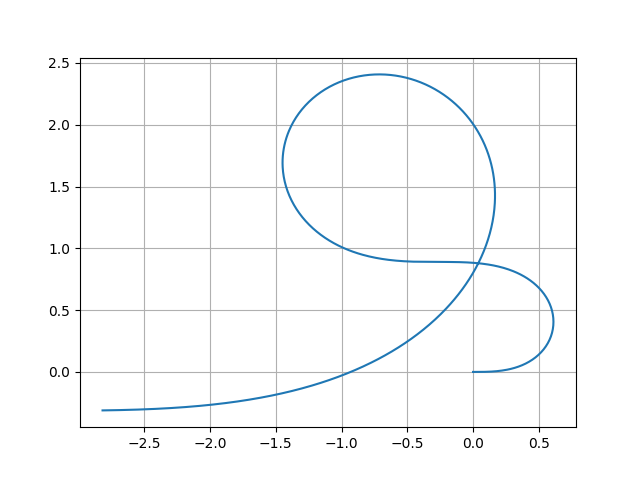
\includegraphics[width = 0.6\textwidth]{Figure_1.png}
    \end{center}

    \item 
    \texttt{For $h = 0.01$ : $K(s=5) = 1.2001127248505328$\\
            For $h = 0.005$ : $K(s=5) = 1.2001135935941987$\\
            For $h = 0.001$ : $K(s=5) = 1.200113871589581$\\
            For $h = 0.0005$ : $K(s=5) = 1.2001138802762434$\\}

    $K(s=5) \approx 1.20011 $\\
    

\end{enumerate}

\item 
\begin{enumerate}
    \item \texttt{The coordinates at t = 2 are: \\$(x,y,z) = (-0.5580567444088435,-0.2720113135900402,0.11995195426460033)$}
    \begin{center}
        \hspace{-50pt}
        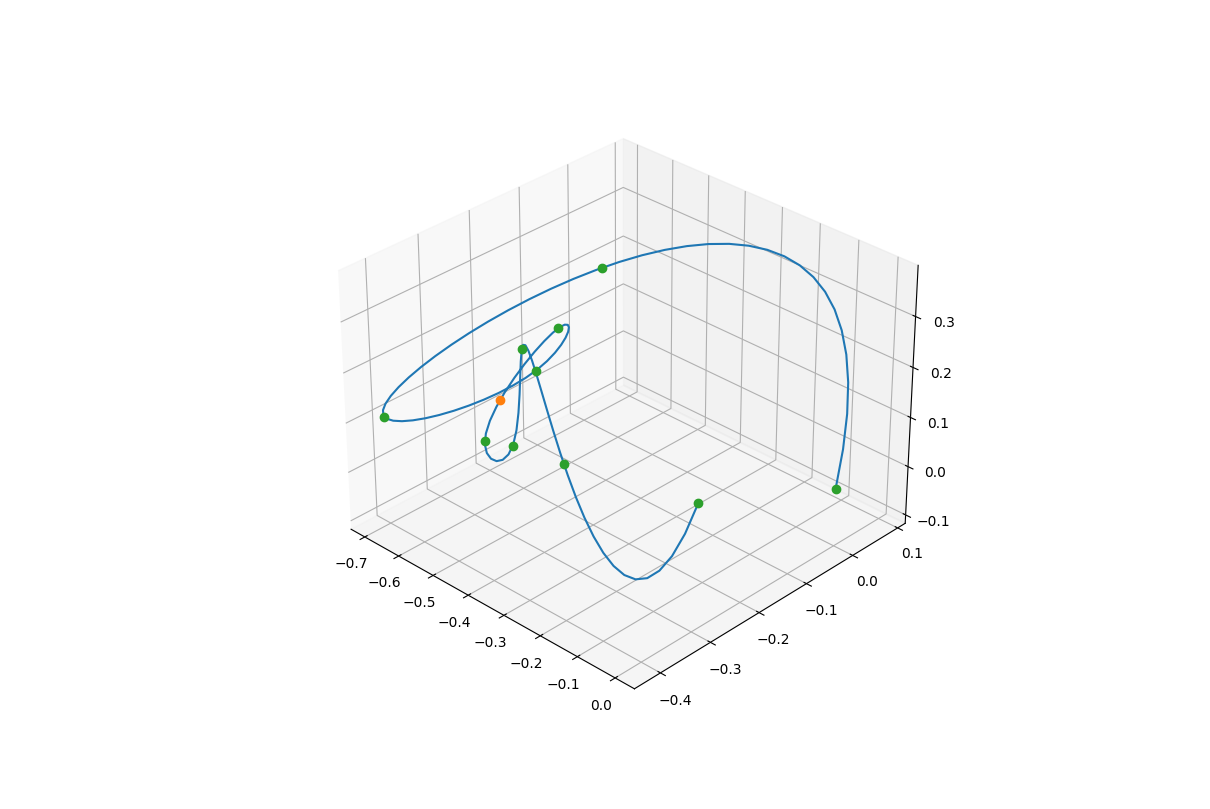
\includegraphics[width = 0.9\textwidth]{Figure_2.png}
    \end{center}

    \item Determine the unit tangent, principal unit normal and binormal vectors at t = 2
    \begin{center}
        \hspace{-50pt}
        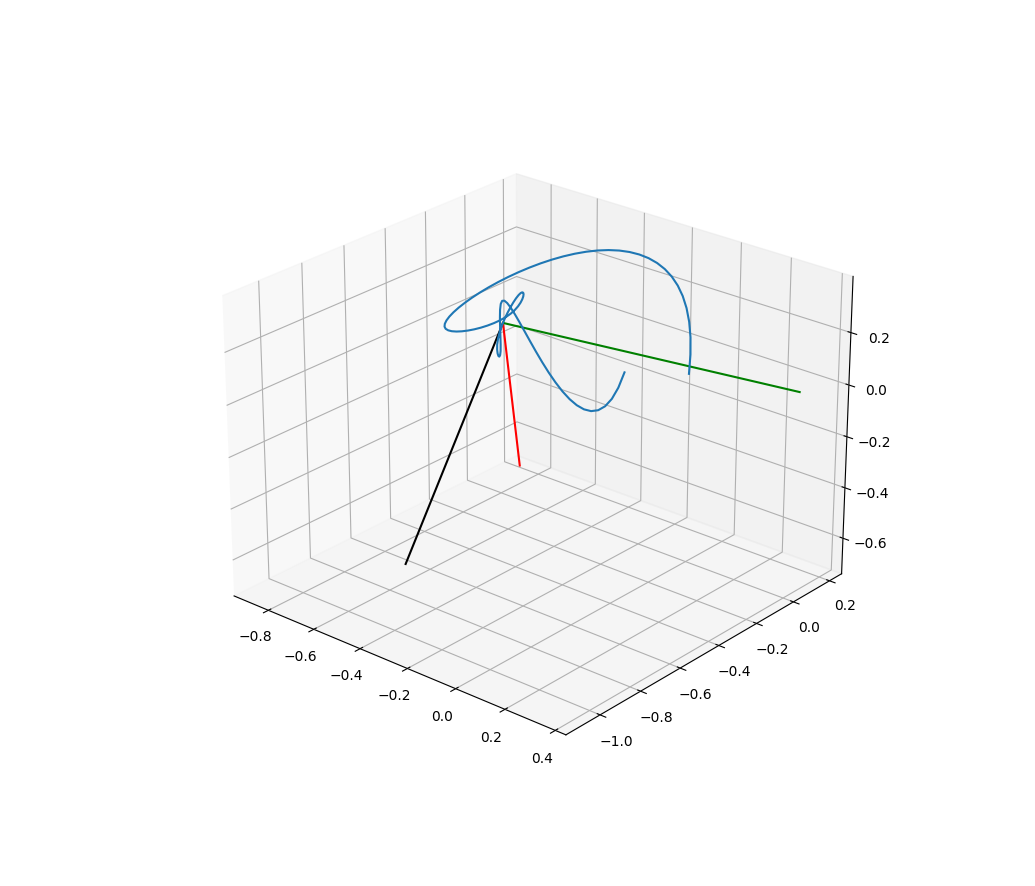
\includegraphics[width = 0.7\textwidth]{Figure_3.png}
    \end{center}
\end{enumerate}

\item 
\begin{enumerate}
    \item The integral evaluates to: 8906.117634354592
    \item The integral evaluates to: 10.787064853079256
\end{enumerate}

\end{enumerate}

\end{enumerate}

\section*{Lab Code}

\inputpython{Lab/lab_questions.py}{1}{1000}

\end{preview}
\end{document}